% ==============================================================================
% MPC WITH EKF
% ==============================================================================

\begin{frame}{MPC with EKF}
    \framesubtitle{State estimation and predictive control}

    \begin{columns}[T,onlytextwidth]
        \begin{column}{0.45\textwidth}
            \begin{block}{Control principle}
                \centering
                \begin{tikzpicture}[
                auto,
                >=Stealth,
                thick,
                node distance=1.4cm and 1.8cm,
                block/.style={
                    draw,
                    rectangle,
                    minimum height=0.7cm,
                    minimum width=1.75cm,
                    align=center,
                    fill=blue!5,
                    rounded corners=2pt,
                    font=\scriptsize
                }
            ]
                \node (ref) {};
                \node[block, below=0.35cm of ref] (mpc)
                    {\textbf{MPC}\\[-1pt]\tiny $\min J(U)$};
                \node[block, right=1.5cm of mpc] (system)
                    {\textbf{Drone} \\ \textbf{System}};
                \node[block, below=1.0cm of mpc] (rnn)
                    {\textbf{RNN model}\\[-1pt]\tiny $(\hat{y},h)$};
                \node[block, below=0.8cm of rnn] (ekf)
                    {\textbf{EKF}\\[-1pt]\tiny $L(y-\hat{y})$};

                \draw[->] (ref) -- node {$r$} (mpc);
                \draw[->] (mpc) -- node[name=u] {$u$} (system);
                \draw[->] (system.south) |- node[pos=0.2, right]
                    {$y$} (ekf.east);
                \draw[->, dashed] (u.center) |- (ekf.30);

                \draw[->] (ekf.west) -- ++(-0.55,0) |- node[pos=0.2, left]
                    {$\hat{h}$} (mpc.west);
                \draw[->] ([xshift=-8pt]mpc.south) --
                    node[left] {$U_{k \dots k+N}$} ([xshift=-8pt]rnn.north);
                \draw[->] ([xshift=8pt]rnn.north) --
                    node[right] {$\hat{y}_{k \dots k+N}$} ([xshift=8pt]mpc.south);
                \end{tikzpicture}
            \end{block}

            % \begin{exampleblock}{Performance}
            %     \begin{itemize}
            %         \item EKF-based state estimation improves feedback.
            %         \item The closed-loop response follows the sinusoidal
            %         reference more closely.
            %         \item The initial transient is reduced compared with the
            %         open-loop response.
            %     \end{itemize}
            % \end{exampleblock}
        \end{column}

        \begin{column}{0.55\textwidth}
            \centering
            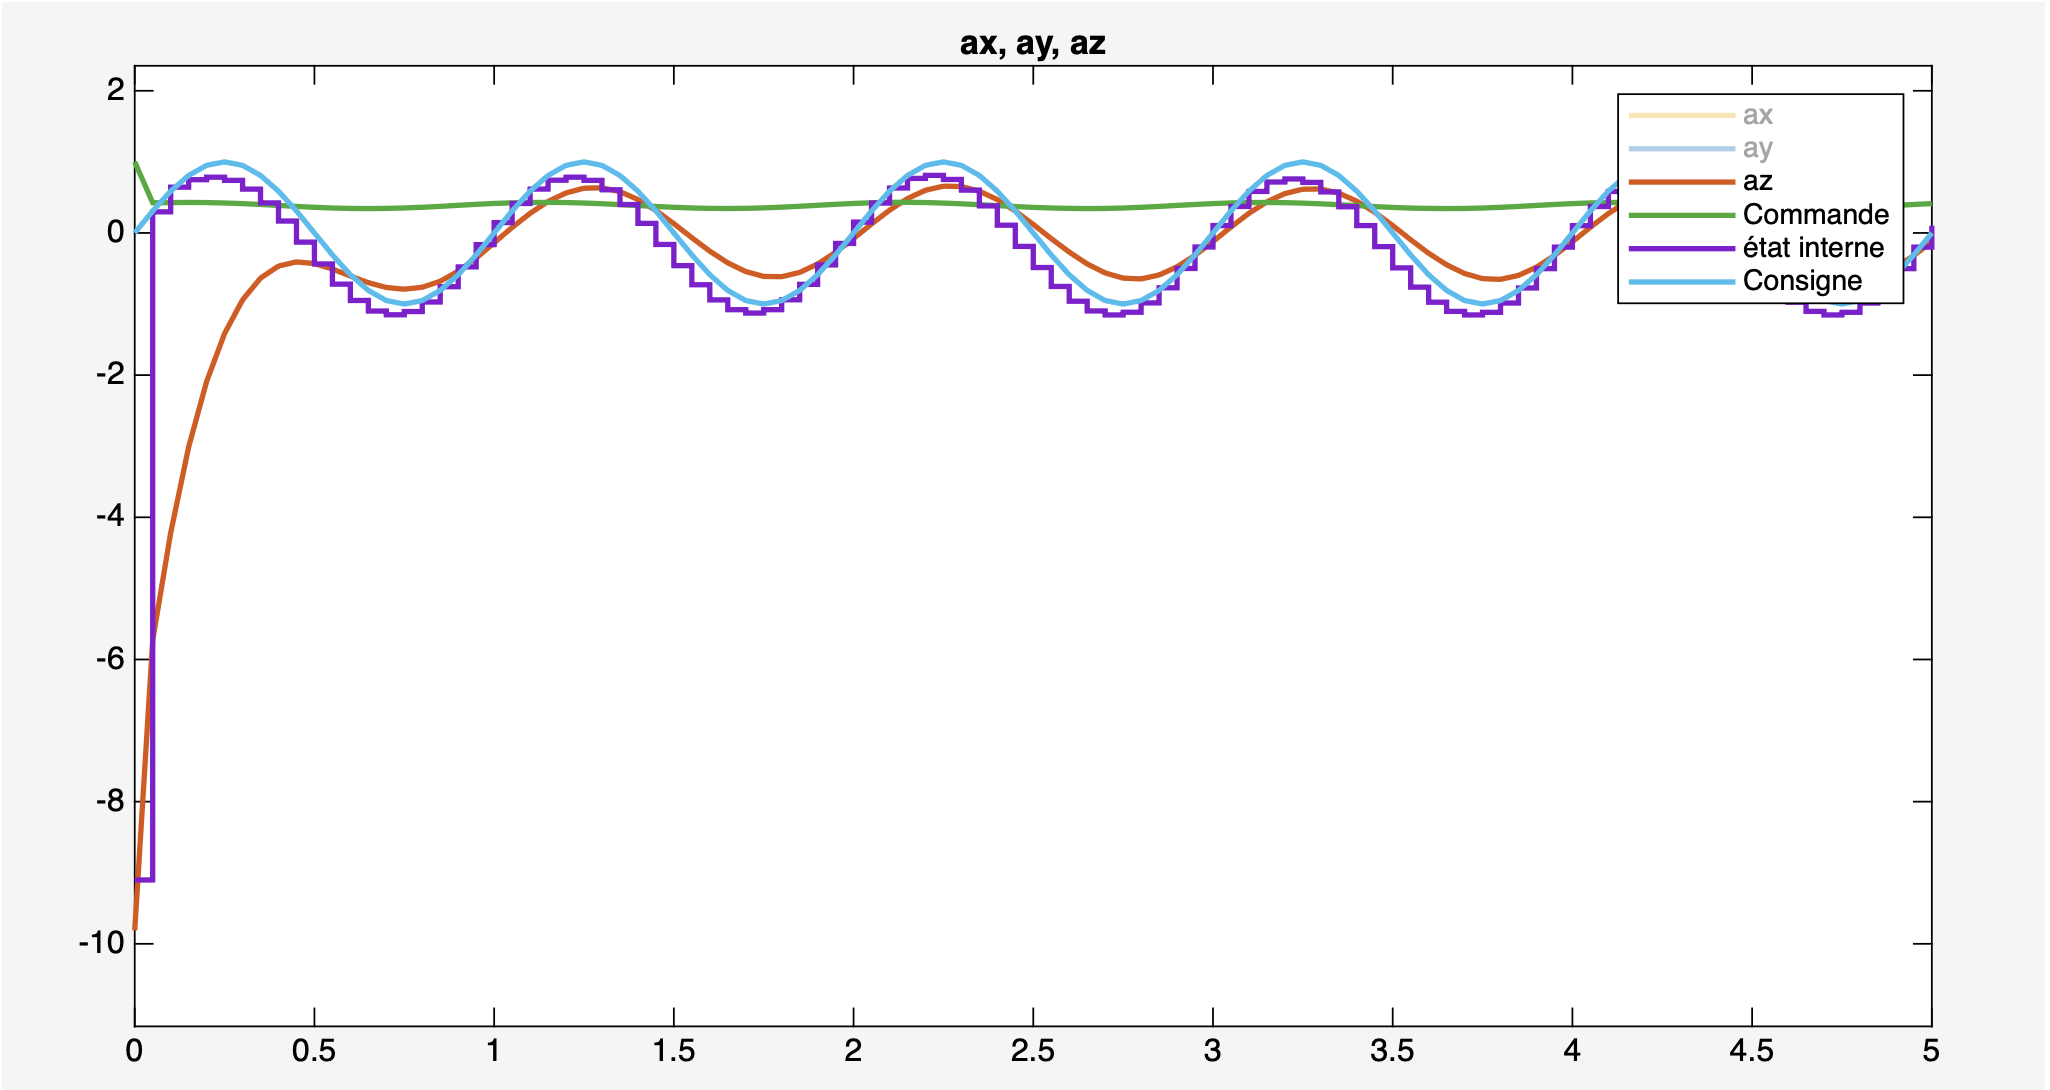
\includegraphics[
                width=\linewidth,
                height=0.38\textheight,
                keepaspectratio
            ]{sinus mpc boucle ouverte.png}

            \vspace{0.12cm}

            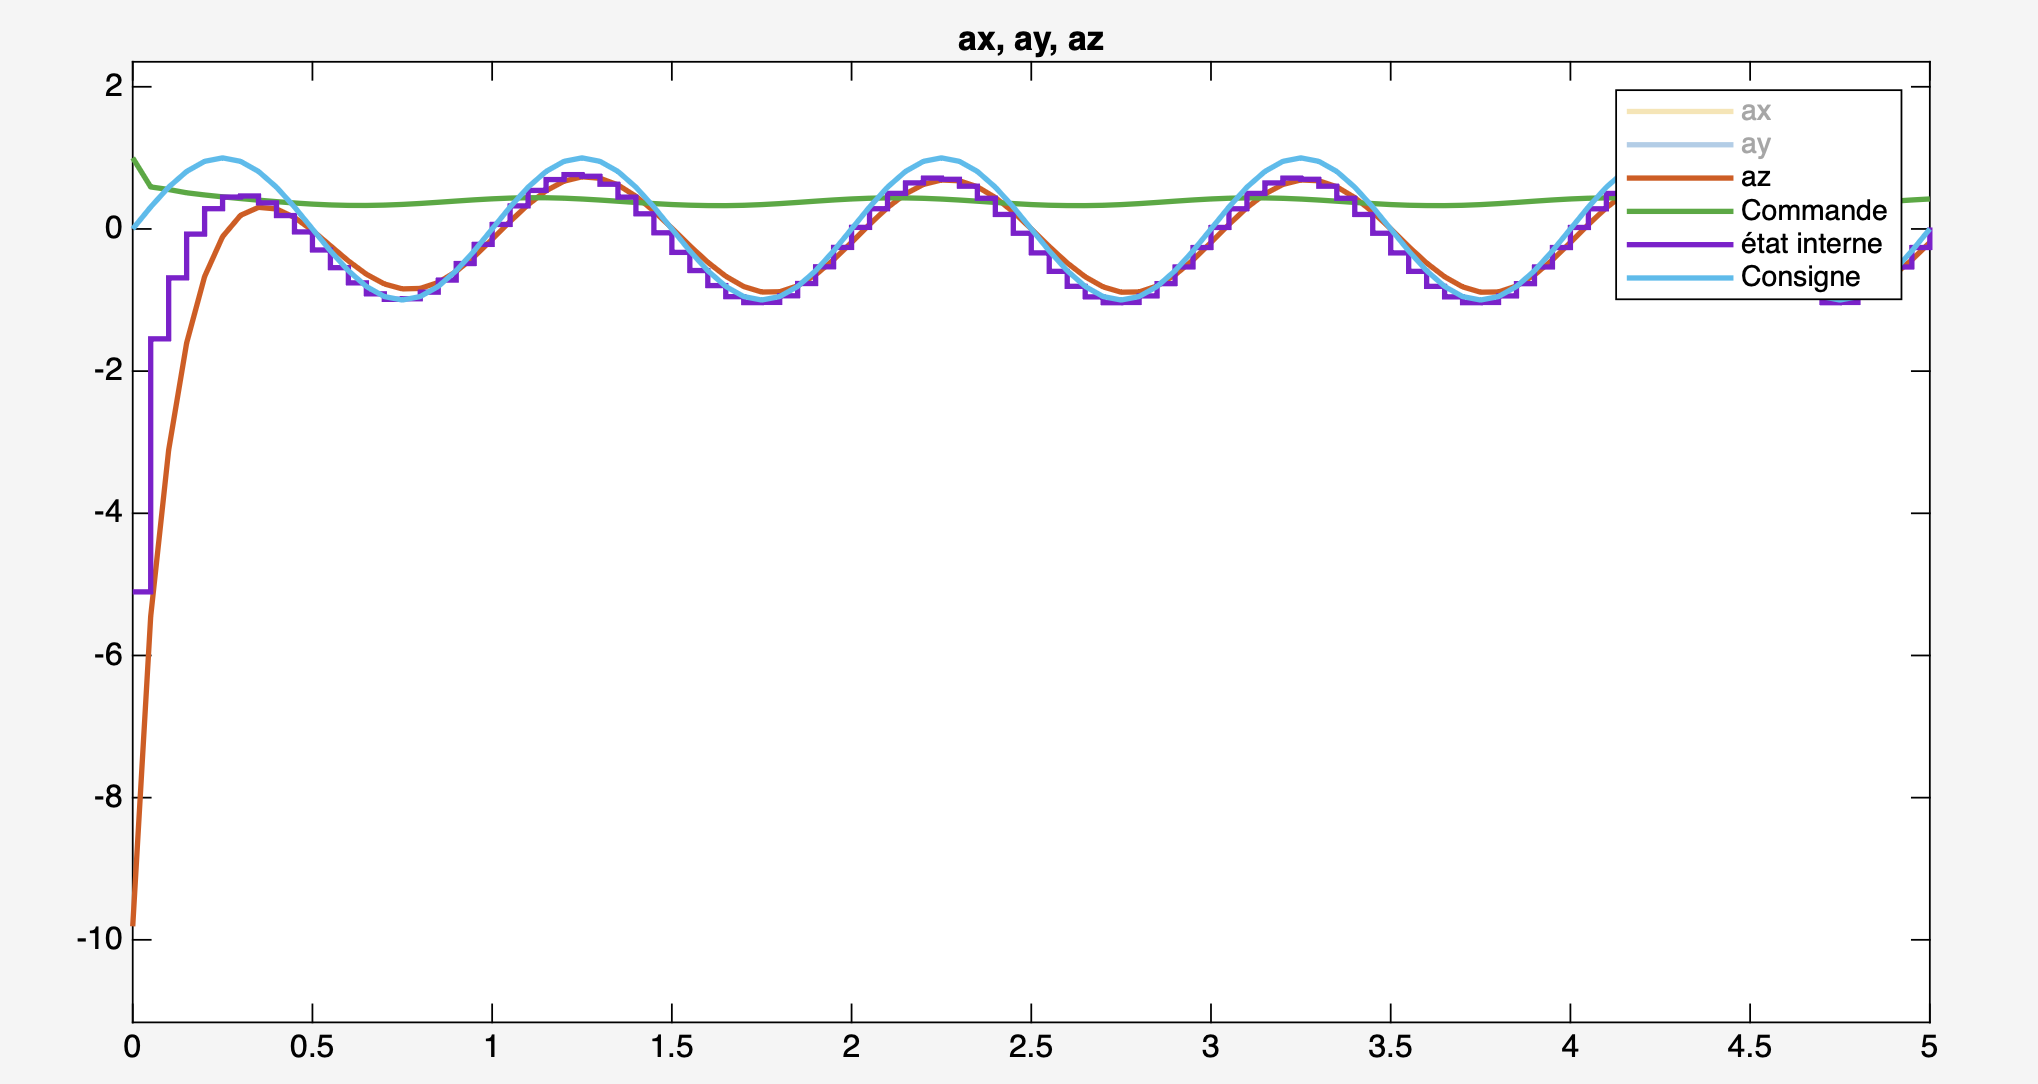
\includegraphics[
                width=\linewidth,
                height=0.38\textheight,
                keepaspectratio
            ]{sinus ekf mpc.png}
        \end{column}
    \end{columns}
\end{frame}
